%% REPLACE sXXXXXXX with your student number
\def\studentNumber{S2569758}


%% START of YOUR ANSWERS
%% Add answers to the questions below, by replacing the text inside the brackets {} for \youranswer{ "Text to be replaced with your answer." }. 
%
% Do not delete the commands for adding figures and tables. Instead fill in the missing values with your experiment results, and replace the images with your own respective figures.
%
% You can generally delete the placeholder text, such as for example the text "Question Figure 2 - Replace the images ..." 
%
% There are 18 TEXT QUESTIONS (a few of the short first ones have their answers added to both the Introduction and the Abstract). Replace the text inside the brackets of the command \youranswer with your answer to the question.
%
% There are also 3 "questions" to replace some placeholder FIGURES with your own, and 3 "questions" asking you to fill in the missing entries in the TABLES provided. 
%
% NOTE! that questions are ordered by the order of appearance of their answers in the text, and not by the order you should tackle them. Specifically, you cannot answer Questions 2, 3, and 4 before concluding all of the relevant experiments and analysis. Similarly, you should fill in the TABLES and FIGURES before discussing the results presented there. 
%
% NOTE! If for some reason you do not manage to produce results for some FIGURES and TABLES, then you can get partial marks by discussing your expectations of the results in the relevant TEXT QUESTIONS (for example Question 8 makes use of Table 1 and Figure 2).
%
% Please refer to the coursework specification for more details.


%% - - - - - - - - - - - - TEXT QUESTIONS - - - - - - - - - - - - 

%% Question 1: Summarise why overfitting is a problem.
\newcommand{\questionOne} {
\youranswer
{In overfitting, the model learns too much about the training data and is unable to generalise its 
learnings for unseen data which leads to poor performance on new data points.}
}

%% Question 2: Summarise the effect increasing width and depth of the architecture had on overfitting.
\newcommand{\questionTwo} {
\youranswer
{Increaseing the depth and width slightly increases the model performance overall but if the either or both the width
and depth are increased by a lot, the model overfits the training data and returns low accuracy scores for any unseen data.}
}

%% Question 3: Summarise what your results show you about the effect of the tested approaches on overfitting and the performance of the trained model
\newcommand{\questionThree} {
\youranswer{Q3}
}

%% Question 4: Give your overall conclusions
\newcommand{\questionFour} {
\youranswer
{complex models can easily overfit the data resulting in low accuracy scores on unseen data points. We can use various techniques like Dropout \& L1/L2 regularisations to ensure that the model doesn't memorise the data and is instead able to generalise the learnings from it.}
}

%% Question 5: Explain in detail, and in your own words, why overfitting is a problem
\newcommand{\questionFive} {
\youranswer
{Overfitting causes a model to start recognising random deviances and noise present in the training data as a regularity rather than learning the underlying patterns.
This poor generalisation leads to the model struggling to capture the trends on unseen data points and hence performing poorly on them. This makes the model less reliable to be used in real world applications.
Another direct consequence of overfitting is that it skews the relationship between variables affecting the interpretability of the model and making it difficult to fix the model.
Overfitting a model also wastes a lot of resources as it would require a lot of computational power to create a model which won't be able to handle new data points very well.}
}

%% Question 6: Explain the relevance of ``network capacity'' to overfitting
\newcommand{\questionSix} {
\youranswer
{Network capacity refers to the ability of the model to learn the general characteristics of the data. When a model is more complex, it starts memorising the data rather than learning the trends from it.
This usually happens when the model has more room than what is needed for capturing the patterns in the data. If the dataset is small or simple, the basic essense of it can be captured with a small model itself.
If in scenarios like this, a complex model is used, the model has the capacity to learn more than the general features of the data and will also start to fit the outliers in the data leading to overfitting on the training set.
Thus it is very important to choose an appropriate model for the data given to us otherwise choosing a complex model with more network capacity will result in overfitting of the data.}
}

%% Question 7: Explain what these figures contain and how the curves evolve, and spot where overfitting occurs. Reason based on the min/max points and velocities (direction and magnitude of change) of the accuracy and error curves
\newcommand{\questionSeven} {
\youranswer
% Describe figure 1a
% all the different width models give very similar accuracy. The models increase the training and validation accuracy rapidly in the first few epochs. After the inital jump, the lines flatten out and marginal improvement is seen in the training accuracy of all the models. On the other hand, 
% the validation accuracy remains similar and doesn't improve much. This is where the overfitting has started, signifying that the model has learned all it could from the training data and now its trying to fit the noise in the data. \par This is further supported 
% by Figure 1b, where we also see the error drop at a rapid rate with the first few epochs. But as the epochs increase, the error on the validation set starts increasing signifying that the model has started to memorise the training data rather than generalising the learnings from it.
{the training accuracy of the model increases rapidly in the first few epochs and then gradually slows down as the epochs continue to run. Even though the validation accuracy also increases at a good rate in the first few epochs, it starts flattening out at a point and then slowly starts to 
decline. This is the point where overfitting has started, stating that the model has learned the training data and is unable to generalise it to the validation data. This is further validated by the graph in Figure 1b which plots the error of the model on the training and validation dataset. 
We can see that the training error reduces rapidly at first and then eventually tends to 0. After a rapid initial decline in the error of the validation set, the error starts increasing at the same time when the accuracy of the validation set starts decreasing. This is due to the fact the model has now overfit 
and is struggling to process unseen data points.}
}

%% Question 8: Present your network width experiment results by using the relevant figure and table
\newcommand{\questionEight} {
\youranswer
{the final validation accuracy of all the models is very close (Figure 2a) indicating that the models performance very similarly. In Figure 2b, if we look at the train and the validation error, we can see the difference in the performance of the models. The training error of the model with 32 hidden units is the highest 
and the one with 128 hidden units is the lowest. This would ideally mean that the model with 128 neurons would be perform the best. But if we look at the validation error, we can see the 128 units model has the highest validation error. This means that model has overfit the training data and is performing relatively
worse on data it has not seen before when compared to the 32 units model. \par From Table 2, we can see that the model with 64 hidden units has the highest validation accuracy and the lowest validation error signifying that the model has learned from the training data and is able to generalise the best on unseen data out of all the 3 models. 
This model is relatively not too complex and is performing better than a model with more width.}
}

%% Question 9: Discuss whether varying width affects the results in a consistent way, and whether the results are expected and match well with the prior knowledge (by which we mean your expectations as are formed from the relevant Theory and literature)
\newcommand{\questionNine} {
\youranswer
{Changing the width of the model gave us a variety of results. We saw that a model with more width (more complex model) is not necessarily the best model for most scenarios. Even though the model might slightly perform better on the training data, it gives a higher error and not a significant increase on the accuracy for new data points.
The results we've achieved also prove the point about the network capacity, where a higher width model has the more than the required capacity to learn the features of the data and thus it starts fitting the outliers to the data leading to overfitting. This won't always be the case as this test was conducted on a relatively simple dataset.
If the data to be processed had more features, we would require a model with more width to learn the underlying patterns in the data. A complex model in this scenario won't overfit because its capacity is being completely utilised in learning the features of the data.}
}

%% Question 10: Present your network depth experiment results by using the relevant figure and table
\newcommand{\questionTen} {
\youranswer
{models of different depth are all capable of classifying classes of EMNIST dataset. From Figure 3a, providing the models with more depth has enabled them to extract features from the data efficiently and give excellent accuracy scores. Irrespective of their depth, in case of validation data, all of them are performing similarly and giving 
accuracy of around 80\% (Table 2). The rise of accuracy is very steep in the first 10 epochs, and then it is slow gradual improvement in training accuracy and barely any change in the validation accuracy. \par The error behaves very differently and gives a good understanding of the models. In Figure 3b, we can see that the error of all the models on 
the training set approaches 0, but on the validation set starts increasing as the epochs increase. This is the point of overfitting; and the magnitude of the error indicates how much the model has learned the training data. The model with the highest depth has the highest capacity and hence has been able to learn the train set the best resulting 
in it having the highest error on the validation set (from Table 2).}
}

%% Question 11: Discuss whether varying depth affects the results in a consistent way, and whether the results are expected and match well with the prior knowledge (by which we mean your expectations as are formed from the relevant Theory and literature)
\newcommand{\questionEleven} {
\youranswer
{Increasing the depth of the model can be helpful in processing large or complex datasets. But in other situations it can turn out to be counter productive and as the model will overfit the data. This is because certain capability is required for the model to process the data, but if the model has more room to capture features, it'll start fitting the 
noise to the dataset. As the depth of the model increases, there are more neurons available which allow the model to extract more features from the dataset allowing it to overfit the training data and result in poor accuracy scores for unseen data. It also becomes computationally expensive to train the model and the resources will be wasted if the model
overfits on the training data. We can tackle the problem of overfitting by using methods like Dropout and Regularisation which penalise the model for generalising too much to the training set preventing overfitting.}
}



%% Question 12: Explain how one could use a combination of L1 and L2 regularisation. Discuss any potential benefits of this approach
\newcommand{\questionTwelve} {
\youranswer{Question 12 - Elastic Net - combo of both L1 and L2 (ridge and lasso)}
}

%% Question 13:
\newcommand{\questionThirteen} {
\youranswer{Question 13 - Explain the experimental details (e.g. hyperparameters), discuss the results in terms of their generalisation performance and overfitting. Select and test the best performing model as part of this analysis.}
}

%% Question 14:
\newcommand{\questionFourteen} {
\youranswer{Question 14 - Assume you were able to run 8 further experiments (8 specific hyperparameter configurations) where you could combine Dropout and L1, and/or Dropout and L2 regularisation. Which 8 runs would you pick and what question(s) would you aim to answer? Make sure you define the experiment setup, including any relevant hyperparameters}
}



%% Question 15:
\newcommand{\questionFifteen} {
\youranswer{Question 15 - Briefly draw your conclusions based on the results from the previous sections (what are the take-away messages?), discussing them in the context of the overall literature, and conclude your report with a recommendation for future directions}
}

%% - - - - - - - - - - - - FIGURES - - - - - - - - - - - - 

%% Question Figure 2:
\newcommand{\questionFigureTwo} {
\youranswer{Question Figure 2 - Replace the images in Figure 2 with figures depicting the accuracy and error, training and validation curves for your experiments varying the number of hidden units.
%
\begin{figure}[t]
    \centering
    \begin{subfigure}{\linewidth}
        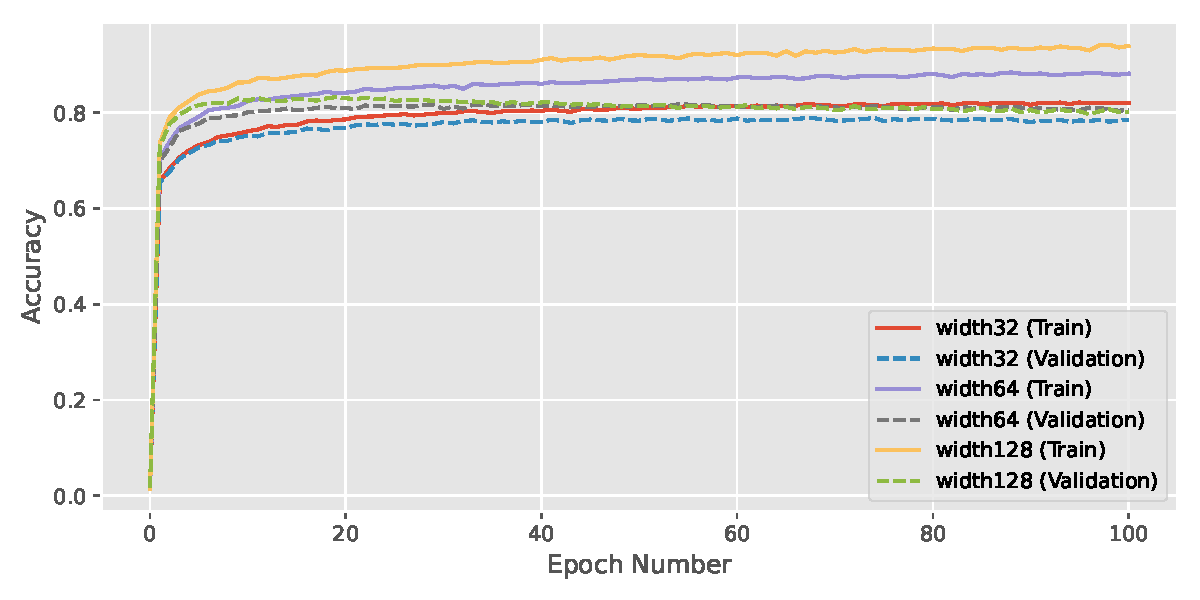
\includegraphics[width=\linewidth]{figures/fig2_acc.pdf}
        \caption{accuracy by epoch}
        \label{fig:width_acccurves}
    \end{subfigure} 
    \begin{subfigure}{\linewidth}
        \centering
        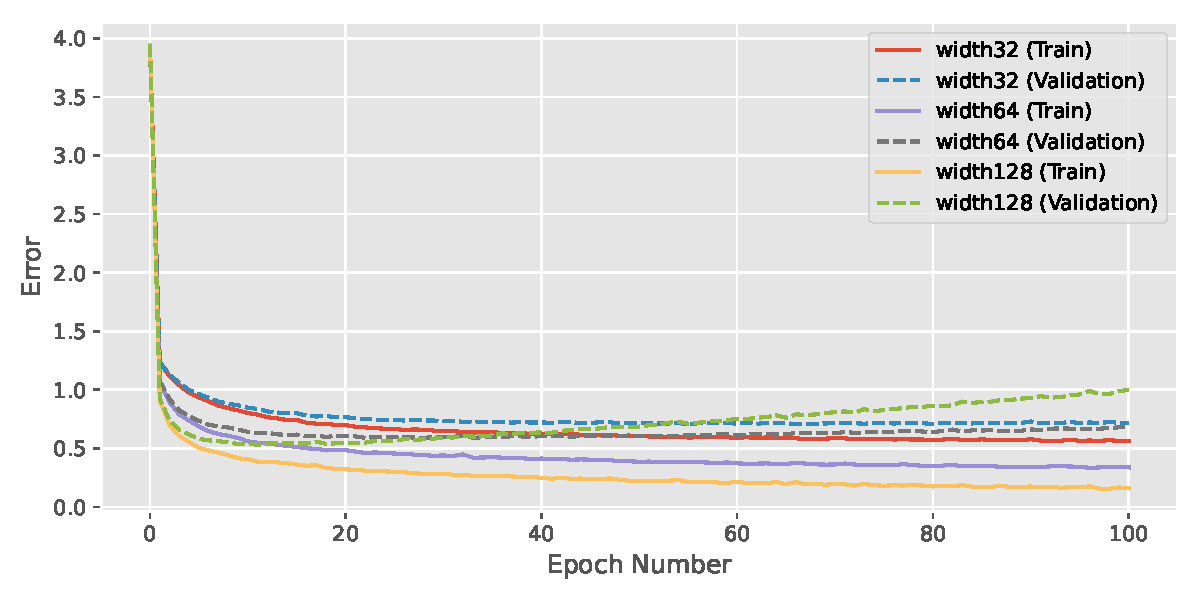
\includegraphics[width=\linewidth]{figures/fig2_err.pdf}
        \caption{error by epoch}
        \label{fig:width_errorcurves}
    \end{subfigure} 
    \caption{Training and validation curves in terms of classification accuracy (a) and cross-entropy error (b) on the EMNIST dataset for different network widths.}
    \label{fig:width}
\end{figure} 
}
}

%% Question Figure 3:
\newcommand{\questionFigureThree} {
\youranswer{Question Figure 3 - Replace these images with figures depicting the accuracy and error, training and validation curves for your experiments varying the number of hidden layers.
%
\begin{figure}[t]
    \centering
    \begin{subfigure}{\linewidth}
        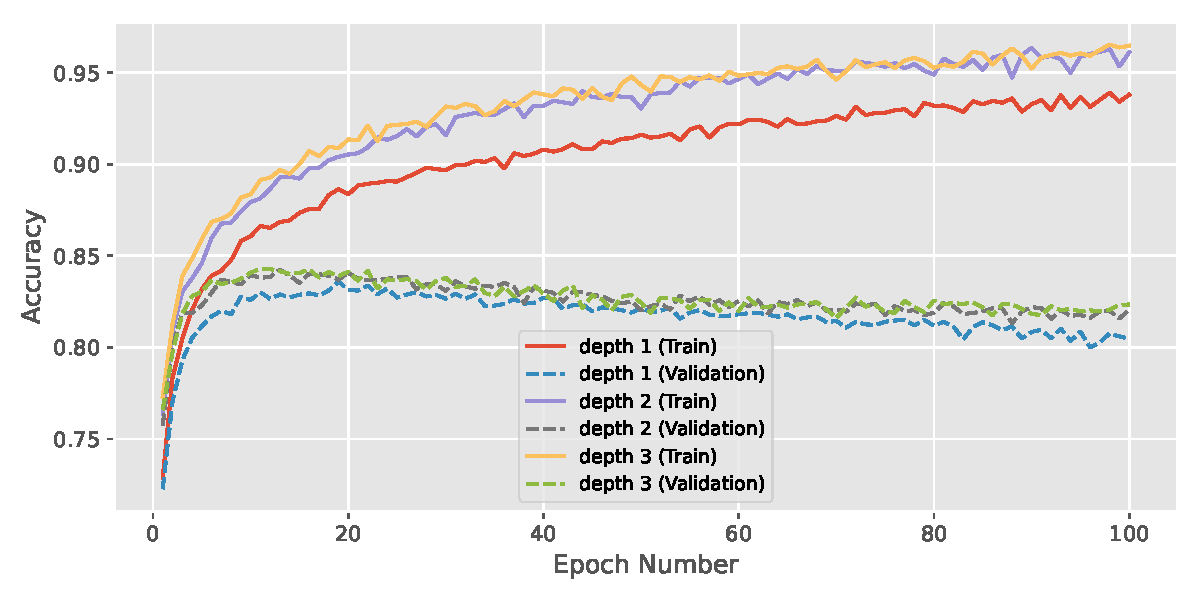
\includegraphics[width=\linewidth]{figures/fig3_acc.pdf}
        \caption{accuracy by epoch}
        \label{fig:depth_acccurves}
    \end{subfigure} 
    \begin{subfigure}{\linewidth}
        \centering
        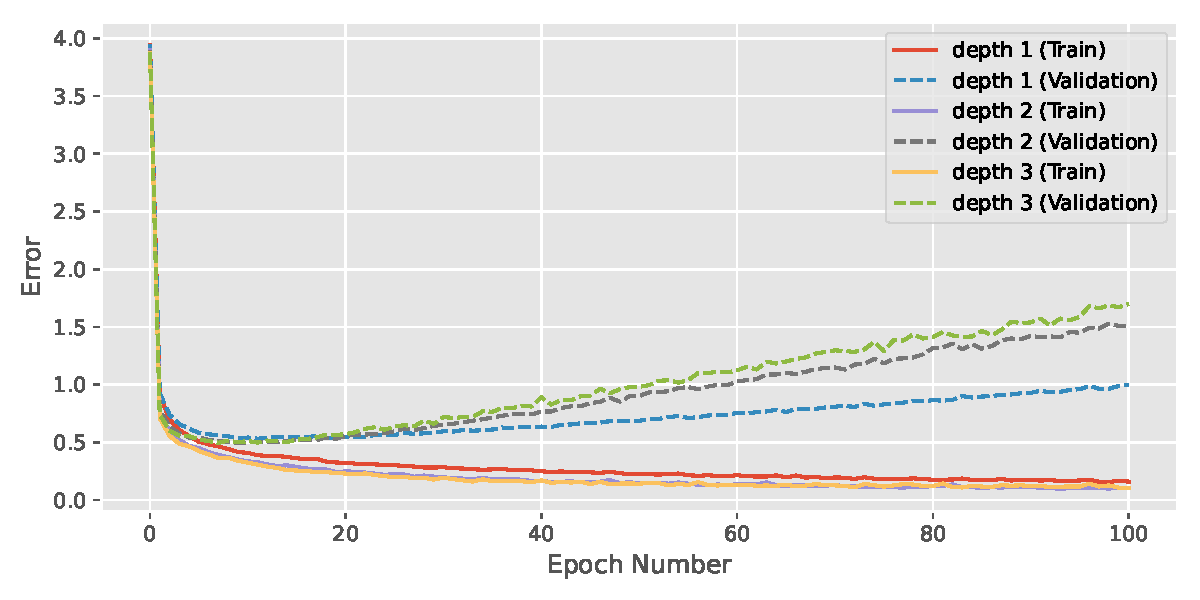
\includegraphics[width=\linewidth]{figures/fig3_err.pdf}
        \caption{error by epoch}
        \label{fig:depth_errorcurves}
    \end{subfigure} 
    \caption{Training and validation curves in terms of classification accuracy (a) and cross-entropy error (b) on the EMNIST dataset for different network depths.}
    \label{fig:depth}
\end{figure} 
}
}

%% Question Figure 4:
\newcommand{\questionFigureFour} {
\youranswer{Question Figure 4 - Replace these images with figures depicting the Validation Accuracy and Generalisation Gap (difference between validation and training error) for each of the experiment results varying the Dropout inclusion rate, and L1/L2 weight penalty depicted in Figure 3 (including any results you have filled in).
%
\begin{figure*}[t]
    \centering
    \begin{subfigure}{.475\linewidth}
        \includegraphics[width=\linewidth]{figures/empty_dropout_plot.png}
        \caption{Accuracy and error by inclusion probability.}
        \label{fig:dropoutrates}
    \end{subfigure} 
    \begin{subfigure}{.475\linewidth}
        \centering
        \includegraphics[width=\linewidth]{figures/empty_wd_plot.png}
        \caption{Accuracy and error by weight penalty.}
        \label{fig:weightrates}
    \end{subfigure} 
    \caption{Accuracy and error by regularisation strength of each method (Dropout and L1/L2 Regularisation).}
    \label{fig:hp_search}
\end{figure*}
}
}

%% - - - - - - - - - - - - TABLES - - - - - - - - - - - - 

%% Question Table 1:
\newcommand{\questionTableOne} {
\youranswer{
Question Table 1 - Fill in Table 1 with the results from your experiments varying the number of hidden units.
%
\begin{table}[t]
    \centering
    \begin{tabular}{c|ccc}
    \toprule
        \# Hidden Units & Val. Acc. & Train Error & Val. Error\\
    \midrule
         32            &    78.9   &  0.563  &   0.705            \\
         64            &    80.9   &  0.345  &   0.809               \\
         128           &    80.5   &  0.163  &   0.805           \\ 
    \bottomrule
    \end{tabular}
    \caption{Validation accuracy (\%) and training/validation error (in terms of cross-entropy error) for varying network widths on the EMNIST dataset.}
    \label{tab:width_exp}
\end{table}
}
}

%% Question Table 2:
\newcommand{\questionTableTwo} {
\youranswer{
Question Table 2 - Fill in Table 2 with the results from your experiments varying the number of hidden layers.
%
\begin{table}[t]
    \centering
    \begin{tabular}{c|ccc}
    \toprule
        \# Hidden Layers & Val. Acc. & Train Error & Val. Error \\
    \midrule
         1               &      80.5      &   0.163 & 0.924               \\
         2               &      82.1      &   0.095 & 1.463                \\
         3               &      82.3      &   0.089 & 1.672                \\ 
    \bottomrule
    \end{tabular}
    \caption{Validation accuracy (\%) and training/validation error (in terms of cross-entropy error) for varying network depths on the EMNIST dataset.}
    \label{tab:depth_exps}
\end{table}
}
}

%% Question Table 3:
\newcommand{\questionTableThree} {
\youranswer{
Question Table 3 - Fill in Table 3 with the results from your experiments for the missing hyperparameter values for each of L1 regularisation, L2 regularisation, and Dropout (use the values shown on the table).
%
\begin{table*}[t]
    \centering
    \begin{tabular}{c|c|ccc}
    \toprule
        Model    &  Hyperparameter value(s) & Validation accuracy & Train Error & Validation Error \\
    \midrule
    \midrule
        Baseline &  -                    &               0.837 &       0.241 &  0.533          \\
    \midrule
        \multirow{4}*{Dropout}
                 & 0.6                   &  80.7                &      0.549 & 0.593     \\
                 & 0.7 & --.- & -.--- & -.---  \\
                 & 0.85 & 85.1 &  0.329 &  0.434 \\
                 & 0.97 & 85.4 &  0.244 & 0.457  \\
    \midrule
        \multirow{4}*{L1 penalty}
                 & 5e-4 & 79.5 & 0.642 & 0.658 \\
                 & 1e-3 & --.- & -.--- & -.--- \\
                 & 5e-3 & 2.41 & 3.850 & 3.850 \\
                 & 5e-2 & 2.20 & 3.850 & 3.850 \\
    \midrule
        \multirow{4}*{L2 penalty}  
                 & 5e-4 & 85.1 & 0.306 & 0.460 \\
                 & 1e-3 & --.- & -.--- & -.--- \\
                 & 5e-3 & 81.3 & 0.586 & 0.607 \\
                 & 5e-2 & 39.2 & 2.258 & 2.256  \\      
    \bottomrule
    \end{tabular}
    \caption{Results of all hyperparameter search experiments. \emph{italics} indicate the best results per series (Dropout, L1 Regularisation, L2 Regularisation) and \textbf{bold} indicates the best overall.}
    \label{tab:hp_search}
\end{table*}
}
}

%% END of YOUR ANSWERS
